\begin{figure*}[t]
\centering
\begin{subfigure}[t]{0.48\textwidth}
  \centering
  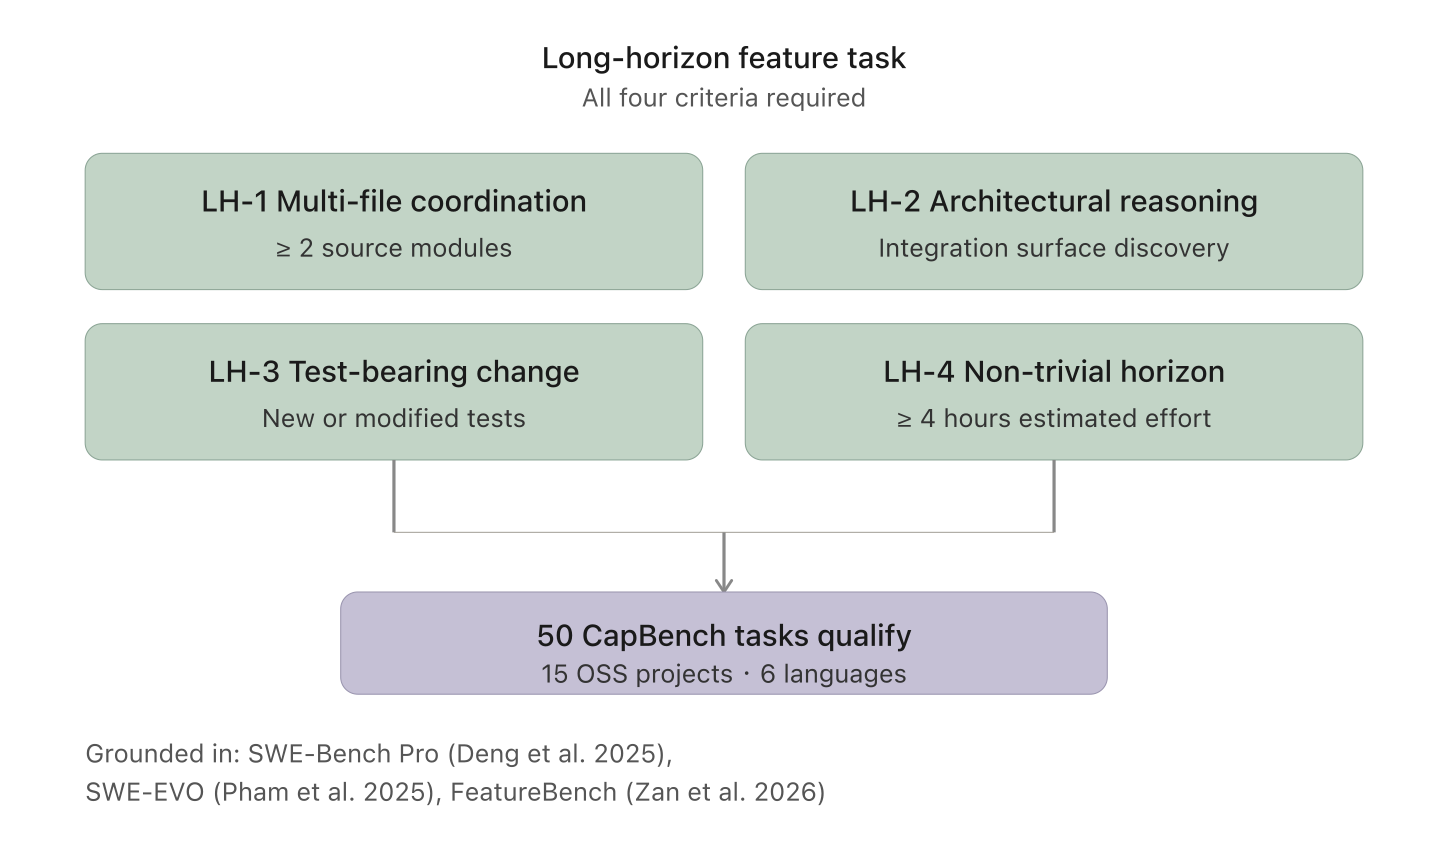
\includegraphics[width=\linewidth]{svg/long_horizon_task_definition.png}
  \caption{Long-horizon task criteria.}
  \label{fig:long-horizon-definition}
\end{subfigure}\hfill
\begin{subfigure}[t]{0.48\textwidth}
  \centering
  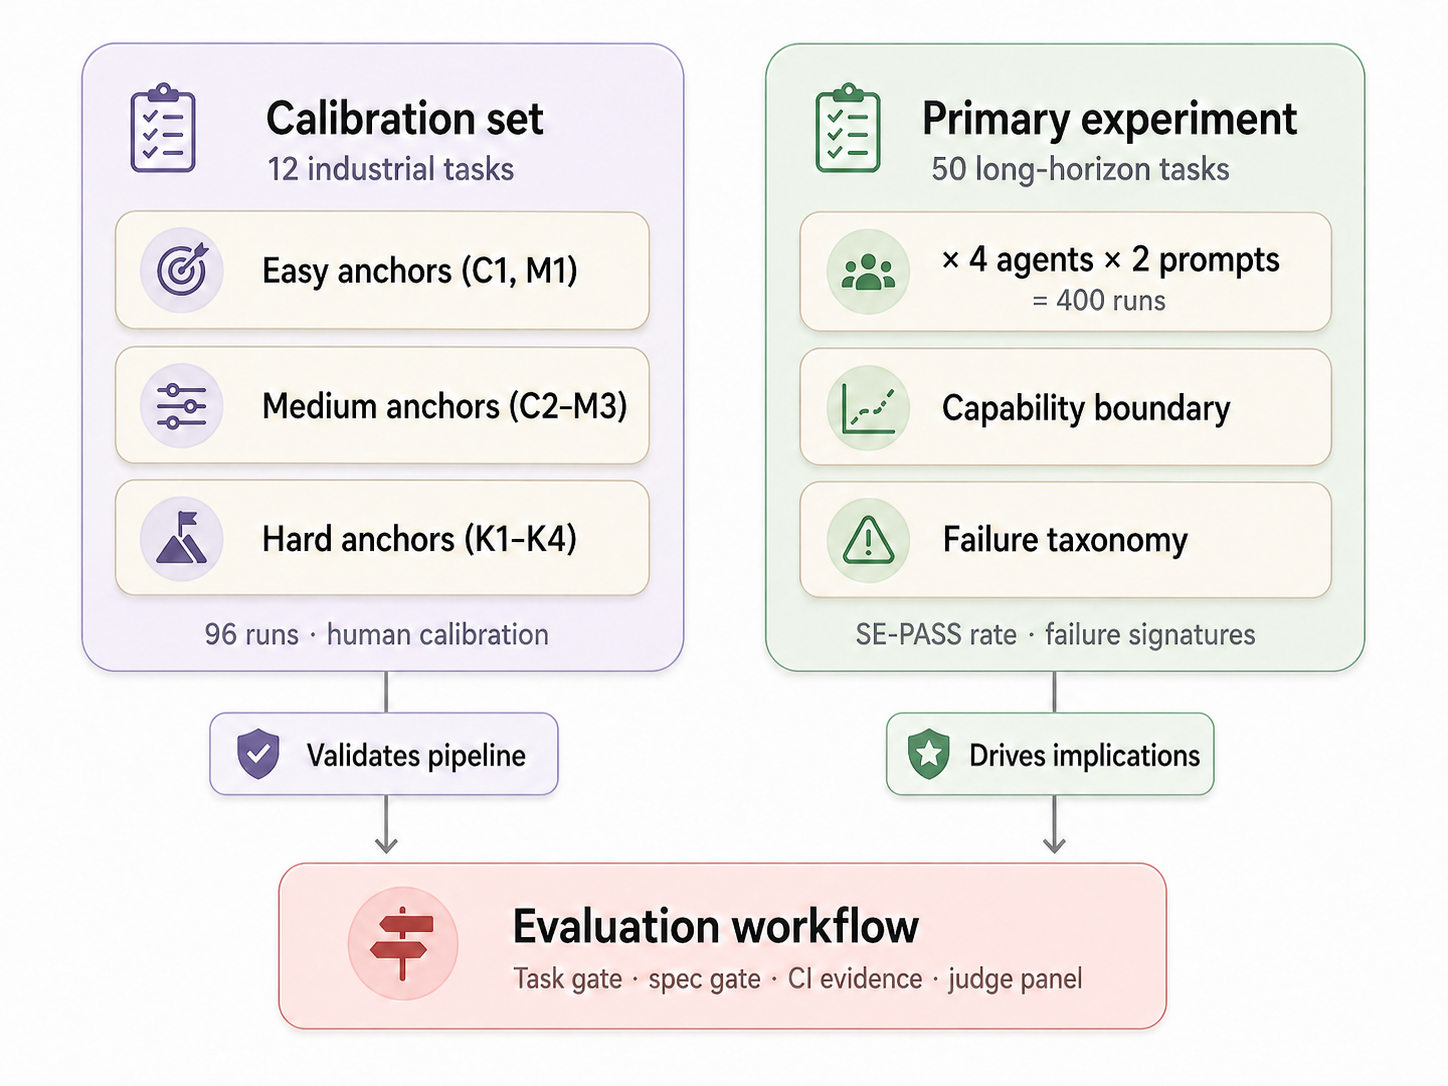
\includegraphics[width=\linewidth]{svg/study_architecture_overview.png}
  \caption{Two-tier study architecture.}
  \label{fig:study-architecture}
\end{subfigure}
\caption{Study framing. Panel~(a) operationalizes long-horizon feature work as multi-file coordination, architecture-aware integration, test-bearing change, and non-trivial implementation horizon. Panel~(b) shows how the 12-task industrial calibration subset validates the scoring pipeline while the 50-task main corpus measures the capability boundary.}
\Description{Two-panel figure. The first panel lists four criteria for long-horizon feature tasks. The second panel shows the calibration subset and primary experiment feeding into evaluation and implications.}
\label{fig:study-overview-panels}
\end{figure*}
